\section{Utility APIs}

\subsection{Byte sized buffers}

\begin{lstlisting}[style=CStyle]
void qBSBuffer_Setup( qBSBuffer_t * const obj, volatile qUINT8_t *buffer, 
                      const size_t length )
\end{lstlisting}

Initialize the byte-sized buffer. \index{\lstinline{qBSBuffer_Setup}}

\subsubsection*{Parameters:}
\begin{itemize}
    \item \lstinline{obj} : A pointer to the byte-sized buffer object
    \item \lstinline{buffer} : Block of memory or array of data.
    \item \lstinline{length} : The size of \lstinline{buffer}(Must be a power of two)
\end{itemize}

\noindent\hrulefill

\begin{lstlisting}[style=CStyle]
qBool_t qBSBuffer_Put( qBSBuffer_t * const obj, const qUINT8_t data )
\end{lstlisting}

Adds an element of data to the byte-sized buffer. \index{\lstinline{qBSBuffer_Put}}

\subsubsection*{Parameters:}
\begin{itemize}
    \item \lstinline{obj} : A pointer to the byte-sized buffer object
    \item \lstinline{data} : The data to be added.
\end{itemize}

\subsubsection*{Return value:}
\lstinline{qTrue} on success, otherwise returns \lstinline{qFalse}.

\noindent\hrulefill

\begin{lstlisting}[style=CStyle]
qBool_t qBSBuffer_Read( qBSBuffer_t * const obj, void *dest, 
                        const size_t n )
\end{lstlisting}

Gets \lstinline{n} data from the byte-sized buffer and removes them. \index{\lstinline{qBSBuffer_Read}}

\subsubsection*{Parameters:}
\begin{itemize}
    \item \lstinline{obj} : A pointer to the byte-sized buffer object
    \item \lstinline{dest} : The location where the data will be written.
\end{itemize}

\subsubsection*{Return value:}
\lstinline{qTrue} on success, otherwise returns \lstinline{qFalse}.

\noindent\hrulefill

\begin{lstlisting}[style=CStyle]
qBool_t qBSBuffer_Get( qBSBuffer_t * const obj, qUINT8_t *dest )
\end{lstlisting}

Gets one data-byte from the front of the byte-sized buffer, and remove it. \index{\lstinline{qBSBuffer_Get}}

\subsubsection*{Parameters:}
\begin{itemize}
    \item \lstinline{obj} : A pointer to the byte-sized buffer object
    \item \lstinline{dest} : The location where the data will be written.
\end{itemize}

\subsubsection*{Return value:}
\lstinline{qTrue} on success, otherwise returns \lstinline{qFalse}.


\noindent\hrulefill

\begin{lstlisting}[style=CStyle]
qUINT8_t qBSBuffer_Peek( const qBSBuffer_t * const obj )
\end{lstlisting}

Looks for one byte from the head of the byte-sized buffer without removing it. \index{\lstinline{qBSBuffer_Peek}}

\subsubsection*{Parameters:}
\begin{itemize}
    \item \lstinline{obj} : A pointer to the byte-sized buffer object
\end{itemize}

\subsubsection*{Return value:}
Byte of data, or zero if nothing in the buffer.

\noindent\hrulefill

\begin{lstlisting}[style=CStyle]
qBool_t qBSBuffer_Empty( const qBSBuffer_t * const obj )
\end{lstlisting}

Query the empty status of the byte-sized buffer. \index{\lstinline{qBSBuffer_Empty}}

\subsubsection*{Parameters:}
\begin{itemize}
    \item \lstinline{obj} : A pointer to the byte-sized buffer object
\end{itemize}

\subsubsection*{Return value:}
\lstinline{qTrue} if the byte-sized buffer is empty, \lstinline{qFalse} if it is not.


\noindent\hrulefill

\begin{lstlisting}[style=CStyle]
qBool_t qBSBuffer_IsFull( const qBSBuffer_t * const obj )
\end{lstlisting}

Query the full status of the byte-sized buffer. \index{\lstinline{qBSBuffer_IsFull}}

\subsubsection*{Parameters:}
\begin{itemize}
    \item \lstinline{obj} : A pointer to the byte-sized buffer object
\end{itemize}

\subsubsection*{Return value:}
\lstinline{qTrue} if the byte-sized buffer is full, \lstinline{qFalse} if it is not.


\noindent\hrulefill

\begin{lstlisting}[style=CStyle]
size_t qBSBuffer_Count( const qBSBuffer_t * const obj )
\end{lstlisting}

Query the number of elements in the byte-sized buffer. \index{\lstinline{qBSBuffer_Count}}

\subsubsection*{Parameters:}
\begin{itemize}
    \item \lstinline{obj} : A pointer to the byte-sized buffer object.
\end{itemize}

\subsubsection*{Return value:}
Number of elements in the byte-sized buffer.



\subsection{Input groups for edge-checking}

\begin{lstlisting}[style=CStyle]
qBool_t qEdgeCheck_Setup( qEdgeCheck_t * const Instance, 
                          const qCoreRegSize_t RegisterSize,
                          const qClock_t DebounceTime )
\end{lstlisting}

Initialize an I/O edge-check instance. \index{\lstinline{qEdgeCheck_Setup}}

\subsubsection*{Parameters:}
\begin{itemize}
    \item \lstinline{Instance} : A pointer to the I/O edge-check object.
    \item \lstinline{RegisterSize} : The specific-core register size: \lstinline{QREG_8BIT}, \lstinline{QREG_16BIT} or \lstinline{QREG_32BIT}(default).
    \item \lstinline{DebounceTime} : The specified time (in epochs) to bypass the bounce of the input nodes.
\end{itemize}

\subsubsection*{Return value:}
\lstinline{qTrue} on success, otherwise returns \lstinline{qFalse}.

\noindent\hrulefill

\begin{lstlisting}[style=CStyle]
qBool_t qEdgeCheck_Add_Node( qEdgeCheck_t * const Instance, 
                             qEdgeCheck_IONode_t * const Node, 
                             void *PortAddress, 
                             const qBool_t PinNumber )
\end{lstlisting}

Inserts an I/O node to the edge-check instance. \index{\lstinline{qEdgeCheck_Add_Node}}

\subsubsection*{Parameters:}
\begin{itemize}
    \item \lstinline{Instance} : A pointer to the I/O edge-check object.
    \item \lstinline{Node} :  A pointer to the input-node object.
    \item \lstinline{PortAddress} : The address of the core PORTx-register to read the levels of the specified \lstinline{PinNumber}.
    \item \lstinline{PinNumber} : The specified pin to read from \lstinline{PortAddress}.
\end{itemize}

\subsubsection*{Return value:}
\lstinline{qTrue} on success, otherwise returns \lstinline{qFalse}.


\noindent\hrulefill

\begin{lstlisting}[style=CStyle]
qBool_t qEdgeCheck_Update( qEdgeCheck_t * const Instance )
\end{lstlisting}

Update the status of all nodes inside the I/O edge-check instance (non-blocking call). \index{\lstinline{qEdgeCheck_Update}}

\subsubsection*{Parameters:}
\begin{itemize}
    \item \lstinline{Instance} : A pointer to the I/O edge-check object.
\end{itemize}

\subsubsection*{Return value:}
\lstinline{qTrue} on success, otherwise returns \lstinline{qFalse}.


\noindent\hrulefill

\begin{lstlisting}[style=CStyle]
qBool_t qEdgeCheck_Get_NodeStatus( const qEdgeCheck_IONode_t * const Node )
\end{lstlisting}

Query the status of the specified input-node. \index{\lstinline{qEdgeCheck_Get_NodeStatus}}

\subsubsection*{Parameters:}
\begin{itemize}
    \item \lstinline{Instance} : A pointer to the I/O edge-check object.
\end{itemize}

\subsubsection*{Return value:}
The status of the input node : \lstinline{qTrue}, \lstinline{qFalse}, \lstinline{qRising}, \lstinline{qFalling} or \lstinline{qUnknown}.


\subsection{Generic lists} \label{qlist}
The provided list implementation uses a generic \textit{doubly-linked} approach in which each node, apart from storing its data, has two link pointers. The first link points to the previous node in the list and the second link, points to the next node in the list. The first node of the list has its previous link pointing to \lstinline{NULL}, similarly, the last node of the list has its next node pointing to \lstinline{NULL}. \\
The list data-structure, referenced through an object of type \lstinline{qList_t} \index{\lstinline{qList_t}} also has a \textit{head} and a \textit{tail} pointer, to allow fast operations on boundary nodes.

\begin{figure}[H]
    \centering
    \tikzset{every picture/.style={line width=0.75pt}} %set default line width to 0.75pt        
    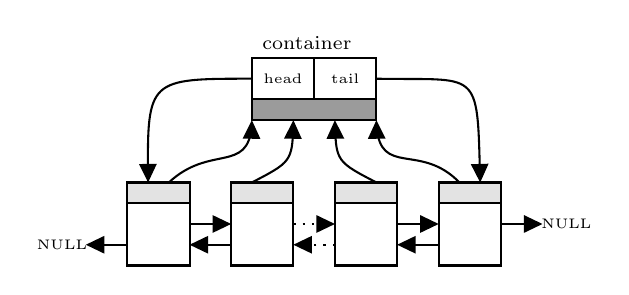
\begin{tikzpicture}[x=0.75pt,y=0.75pt,yscale=-1,xscale=1]
        \draw   (200,110) -- (230,110) -- (230,150) -- (200,150) -- cycle ;
        \draw    (230,130) -- (247,130) ;
        \draw [shift={(250,130)}, rotate = 180] [fill={rgb, 255:red, 0; green, 0; blue, 0 }  ][line width=0.08]  [draw opacity=0] (8.93,-4.29) -- (0,0) -- (8.93,4.29) -- cycle    ;
        \draw    (200,140) -- (183,140) ;
        \draw [shift={(180,140)}, rotate = 360] [fill={rgb, 255:red, 0; green, 0; blue, 0 }  ][line width=0.08]  [draw opacity=0] (8.93,-4.29) -- (0,0) -- (8.93,4.29) -- cycle    ;
        \draw   (250,110) -- (280,110) -- (280,150) -- (250,150) -- cycle ;
        \draw  [dash pattern={on 0.84pt off 2.51pt}]  (280,130) -- (297,130) ;
        \draw [shift={(300,130)}, rotate = 180] [fill={rgb, 255:red, 0; green, 0; blue, 0 }  ][line width=0.08]  [draw opacity=0] (8.93,-4.29) -- (0,0) -- (8.93,4.29) -- cycle    ;
        \draw    (250,140) -- (233,140) ;
        \draw [shift={(230,140)}, rotate = 360] [fill={rgb, 255:red, 0; green, 0; blue, 0 }  ][line width=0.08]  [draw opacity=0] (8.93,-4.29) -- (0,0) -- (8.93,4.29) -- cycle    ;
        \draw   (300,110) -- (330,110) -- (330,150) -- (300,150) -- cycle ;
        \draw    (330,130) -- (347,130) ;
        \draw [shift={(350,130)}, rotate = 180] [fill={rgb, 255:red, 0; green, 0; blue, 0 }  ][line width=0.08]  [draw opacity=0] (8.93,-4.29) -- (0,0) -- (8.93,4.29) -- cycle    ;
        \draw  [dash pattern={on 0.84pt off 2.51pt}]  (300,140) -- (283,140) ;
        \draw [shift={(280,140)}, rotate = 360] [fill={rgb, 255:red, 0; green, 0; blue, 0 }  ][line width=0.08]  [draw opacity=0] (8.93,-4.29) -- (0,0) -- (8.93,4.29) -- cycle    ;
        \draw   (350,110) -- (380,110) -- (380,150) -- (350,150) -- cycle ;
        \draw    (380,130) -- (397,130) ;
        \draw [shift={(400,130)}, rotate = 180] [fill={rgb, 255:red, 0; green, 0; blue, 0 }  ][line width=0.08]  [draw opacity=0] (8.93,-4.29) -- (0,0) -- (8.93,4.29) -- cycle    ;
        \draw    (350,140) -- (333,140) ;
        \draw [shift={(330,140)}, rotate = 360] [fill={rgb, 255:red, 0; green, 0; blue, 0 }  ][line width=0.08]  [draw opacity=0] (8.93,-4.29) -- (0,0) -- (8.93,4.29) -- cycle    ;
        \draw   (260,50) -- (290,50) -- (290,70) -- (260,70) -- cycle ;
        \draw    (320,60) .. controls (369.74,60.99) and (368.55,54.07) .. (369.93,107.52) ;
        \draw [shift={(370,110)}, rotate = 268.47] [fill={rgb, 255:red, 0; green, 0; blue, 0 }  ][line width=0.08]  [draw opacity=0] (8.93,-4.29) -- (0,0) -- (8.93,4.29) -- cycle    ;
        \draw    (260,60) .. controls (210.51,60) and (209.52,60) .. (209.97,107.06) ;
        \draw [shift={(210,110)}, rotate = 269.43] [fill={rgb, 255:red, 0; green, 0; blue, 0 }  ][line width=0.08]  [draw opacity=0] (8.93,-4.29) -- (0,0) -- (8.93,4.29) -- cycle    ;
        \draw   (290,50) -- (320,50) -- (320,70) -- (290,70) -- cycle ;
        \draw  [fill={rgb, 255:red, 155; green, 155; blue, 155 }  ,fill opacity=1 ] (260,70) -- (320,70) -- (320,80) -- (260,80) -- cycle ;
        \draw    (220,110) .. controls (239.78,91.53) and (258.17,105.78) .. (259.88,82.67) ;
        \draw [shift={(260,80)}, rotate = 451.07] [fill={rgb, 255:red, 0; green, 0; blue, 0 }  ][line width=0.08]  [draw opacity=0] (8.93,-4.29) -- (0,0) -- (8.93,4.29) -- cycle    ;
        \draw    (260,110) .. controls (278.52,100.36) and (279.45,99.88) .. (279.93,82.83) ;
        \draw [shift={(280,80)}, rotate = 451.44] [fill={rgb, 255:red, 0; green, 0; blue, 0 }  ][line width=0.08]  [draw opacity=0] (8.93,-4.29) -- (0,0) -- (8.93,4.29) -- cycle    ;
        \draw    (320,110) .. controls (301.47,100.36) and (300.55,99.88) .. (300.07,82.83) ;
        \draw [shift={(300,80)}, rotate = 448.56] [fill={rgb, 255:red, 0; green, 0; blue, 0 }  ][line width=0.08]  [draw opacity=0] (8.93,-4.29) -- (0,0) -- (8.93,4.29) -- cycle    ;
        \draw    (360,110) .. controls (341.18,90.56) and (321.9,107.58) .. (320.12,82.86) ;
        \draw [shift={(320,80)}, rotate = 449.01] [fill={rgb, 255:red, 0; green, 0; blue, 0 }  ][line width=0.08]  [draw opacity=0] (8.93,-4.29) -- (0,0) -- (8.93,4.29) -- cycle    ;
        \draw  [fill={rgb, 255:red, 210; green, 210; blue, 210 }  ,fill opacity=0.62 ] (200,110) -- (230,110) -- (230,120) -- (200,120) -- cycle ;
        \draw  [fill={rgb, 255:red, 210; green, 210; blue, 210 }  ,fill opacity=0.62 ] (250,110) -- (280,110) -- (280,120) -- (250,120) -- cycle ;
        \draw  [fill={rgb, 255:red, 210; green, 210; blue, 210 }  ,fill opacity=0.62 ] (300,110) -- (330,110) -- (330,120) -- (300,120) -- cycle ;
        \draw  [fill={rgb, 255:red, 210; green, 210; blue, 210 }  ,fill opacity=0.62 ] (350,110) -- (380,110) -- (380,120) -- (350,120) -- cycle ;
        \draw (275,60) node  [font=\tiny] [align=left] {\lstinline{head}};
        \draw (305,60) node  [font=\tiny] [align=left] {\lstinline{tail}};
        \draw (286.5,43) node  [font=\scriptsize] [align=left] {container};
        \draw (168.5,140) node  [font=\tiny] [align=left] {\lstinline{NULL}};
        \draw (411.5,130) node  [font=\tiny] [align=left] {\lstinline{NULL}};
    \end{tikzpicture}
    \caption{Doubly-linked list implementation}
    \label{fig:qlistsfigure}
\end{figure}

Nodes should be an user-defined data structure of any number of members, however, they must be specially defined to be compatible with the provided APIs. All the user-defined nodes must have the \lstinline{qNode_MinimalFields} definition on top of the structure. An example is shown below:
\medskip

\begin{lstlisting}[style=CStyle]
typedef struct{
    qNode_MinimalFields; /*< required for lists*/
    int a;
    int b;
    float y;
}userdata_t;
\end{lstlisting}

With this special type definition on all custom data, the application writer can take advantage of this powerful data structure. The following APIs are provided for lists management:

\noindent\hrulefill


\begin{lstlisting}[style=CStyle]
void qList_Initialize( qList_t * const list )
\end{lstlisting}

Must be called before a list is used.  This initializes all the members of the 
list object. \index{\lstinline{qList_Initialize}}

\subsubsection*{Parameters:}
\begin{itemize}
    \item \lstinline{list} : Pointer to the list being initialised. 
\end{itemize}

\noindent\hrulefill

\begin{lstlisting}[style=CStyle]
qBool_t qList_Insert( qList_t *const list, void * const node, 
                      const qList_Position_t position ){
\end{lstlisting}

Insert an item into the list. \index{\lstinline{qList_Insert}}

\subsubsection*{Parameters:}
\begin{itemize}
    \item \lstinline{list} : Pointer to the list. 
    \item \lstinline{node} : A pointer to the node to be inserted.
    \item \lstinline{position} : The position where the node will be inserted. Could be \lstinline{qList_AtFront}, \lstinline{qList_AtBack} or any other index number where the node will be inserted after.
    
    \textit{Note}: If the index exceeds the size of the list, the node will be inserted at the back.
    
    \textit{Note}: If the list is empty, the node will be inserted as the first item.
\end{itemize}

\subsubsection*{Return value:}
\lstinline{qTrue} if the item was successfully added to the list, otherwise returns \lstinline{qFalse}. 

\noindent\hrulefill

\begin{lstlisting}[style=CStyle]
void* qList_Remove( qList_t * const list, void * const node, 
                    const qList_Position_t position )
\end{lstlisting}

Remove an item from the list. \index{\lstinline{qList_Remove}}

\subsubsection*{Parameters:}
\begin{itemize}
    \item \lstinline{list} : Pointer to the list. 
    \item \lstinline{node} : A pointer to the node to be deleted (to ignore pass \lstinline{NULL} ).
    \item \lstinline{position} : The position of the node that will be deleted. Could be \lstinline{qList_AtFront}, \lstinline{qList_AtBack} or any other index number.
    
    \textit{Note}: If the \lstinline{node} argument is supplied, the removal will be only effective if the data is member of the list. If ignored or the data is not a member of the list, this function will use the \lstinline{position} instead as index for removal.
    
    \textit{Note}: If the index exceeds the size of the list, the last node  will be removed.
\end{itemize}

\subsubsection*{Return value:}
A pointer to the removed node. \lstinline{NULL} if removal can be performed.

\noindent\hrulefill

\begin{lstlisting}[style=CStyle]
qBool_t qList_IsMember( const qList_t *const list, const void *const node )
\end{lstlisting}

Check if the node is member of the list. \index{\lstinline{qList_IsMember}}

\subsubsection*{Parameters:}
\begin{itemize}
    \item \lstinline{list} : Pointer to the list. 
    \item \lstinline{node} : A pointer to the node .
\end{itemize}

\subsubsection*{Return value:}
\lstinline{qTrue} if the node belongs to the list, \lstinline{qFalse} if it is not.

\noindent\hrulefill

\begin{lstlisting}[style=CStyle]
void* qList_GetFront( const qList_t *const list ){
\end{lstlisting}

Get a pointer to the front item of the list. \index{\lstinline{qList_GetFront}}

\subsubsection*{Parameters:}
\begin{itemize}
    \item \lstinline{list} : Pointer to the list. 
\end{itemize}

\subsubsection*{Return value:}
A pointer to the front node. \lstinline{NULL} if the list is empty.

\noindent\hrulefill

\begin{lstlisting}[style=CStyle]
void* qList_GetBack( const qList_t *const list )
\end{lstlisting}

Get a pointer to the back item of the list. \index{\lstinline{qList_GetBack}}

\subsubsection*{Parameters:}
\begin{itemize}
    \item \lstinline{list} : Pointer to the list. 
\end{itemize}

\subsubsection*{Return value:}
A pointer to the front node. \lstinline{NULL} if the list is empty.


\noindent\hrulefill

\begin{lstlisting}[style=CStyle]
qBool_t qList_IsEmpty( const qList_t * const list )
\end{lstlisting}

Check if the list is empty. \index{\lstinline{qList_IsEmpty}}

\subsubsection*{Parameters:}
\begin{itemize}
    \item \lstinline{list} : Pointer to the list. 
\end{itemize}

\subsubsection*{Return value:}
\lstinline{qTrue} if the list is empty, \lstinline{qFalse} if it is not.


\noindent\hrulefill

\begin{lstlisting}[style=CStyle]
size_t qList_Length( const qList_t * const list )
\end{lstlisting}

Get the number of items inside the list. \index{\lstinline{qList_Length}}

\subsubsection*{Parameters:}
\begin{itemize}
    \item \lstinline{list} : Pointer to the list. 
\end{itemize}

\subsubsection*{Return value:}
The number of items of the list. 

\noindent\hrulefill

\begin{lstlisting}[style=CStyle]
qBool_t qList_Move( qList_t *const destination, qList_t *const source, 
                    const qList_Position_t position )
\end{lstlisting} \index{\lstinline{qList_Move}}

Moves(or merge) the entire list pointed by \lstinline{source} to the list pointed by \lstinline{destination} at location specified by \lstinline{position}. 
After the move operation, this function leaves empty the list pointed by \lstinline{source}.

\subsubsection*{Parameters:}
\begin{itemize}
    \item \lstinline{destination} : Pointer to the list where the \lstinline{source} nodes are to be moved. 
    \item \lstinline{source} : Pointer to the source list to be moved.
    \item \lstinline{position} : The position where \lstinline{source} list will be inserted. Could be \lstinline{qList_AtFront}, \lstinline{qList_AtBack} or any other index number where the list will be inserted after.
\end{itemize}

\subsubsection*{Return value:}
\lstinline{qTrue} if the move operation is performed successfully, otherwise  returns \lstinline{qFalse}.  

\noindent\hrulefill

\begin{lstlisting}[style=CStyle]
qBool_t qList_ForEach( qList_t *const list, qList_NodeFcn_t Fcn, 
                       void *arg, qList_Direction_t dir, void *NodeOffset )
\end{lstlisting} \index{\lstinline{qList_ForEach}}

Operate on each element of the list.

\subsubsection*{Parameters:}
\begin{itemize}
    \item \lstinline{list} : Pointer to the list.
    \item \lstinline{Fcn} : The function to perform over the node. 
                            
                            Should have this prototype:
                            
                            \lstinline{ qBool_t Function( void* Node, void *arg, qList_WalkStage_t stage ) }
                            
                            where the \lstinline{stage} argument indicates the loop progress and should be checked by the application writer to perform the specific operations over the list. This variable can take the following values:
                            
                            \begin{itemize}
                                \item \lstinline{QLIST_WALKINIT} : When the loop is about to start. In this case, A \lstinline{NULL} value will be passed in the node pointer.
                                \item \lstinline{QLIST_WALKTHROUGH} : When the loop is traversing the list.
                                \item \lstinline{QLIST_WALKEND} :  When the loop has finished. In this case, A \lstinline{NULL} value will be passed in the node pointer
                            \end{itemize}
                            
                            By default, \lstinline{Function} should return \lstinline{qFalse}. If a \lstinline{qTrue} value is returned, the walk through loop will be terminated.
    \item \lstinline{arg} : Argument passed to \lstinline{Fcn}.
    \item \lstinline{dir} : Use one of the following options:
                            \begin{itemize}
                                \item \lstinline{QLIST_FORWARD} : to walk through the list forwards.
                                \item \lstinline{QLIST_BACKWARD} to walk through the list backwards.
                            \end{itemize}
    \item \lstinline{NodeOffset} : If available, the list walk through will start from this node.  
                   To ignore, pass \lstinline{NULL}.
\end{itemize}

\subsubsection*{Return value:}
\lstinline{qTrue} if the walk through was early terminated, otherwise returns \lstinline{qFalse}.

\noindent\hrulefill

\begin{lstlisting}[style=CStyle]
qBool_t qList_Sort( qList_t * const list, 
                    qBool_t (*CompareFcn)(const void *n1, const void *n2) ) 
\end{lstlisting} \index{\lstinline{qList_Sort}}

Sort the double linked list using the \lstinline{CompareFcn} function to 
determine the order.
The sorting algorithm used by this function compares pairs of adjacent nodes by calling the specified \lstinline{CompareFcn} function with pointers to them as arguments. The sort is performed only modifying node's links without data swapping, improving performance if nodes have a large storage.

\textit{Note:} The function modifies the content of the list by reordering its 
elements as defined by \lstinline{CompareFcn}.

\subsubsection*{Parameters:}
\begin{itemize}
    \item \lstinline{list} : Pointer to the list. 
    \item \lstinline{CompareFcn} : Pointer to a function that compares two nodes.
                    This function is called repeatedly by \lstinline{qList_Sort} to compare two nodes. It shall follow the following prototype:
                    \lstinline{qBool_t (*CompareFcn)(void *node1, void *node2)}
                    
                    Taking two pointers as arguments (both converted to (\lstinline{const void*}). The function defines the order of the elements by returning a Boolean data, where a \lstinline{qTrue} value indicates that element pointed by \lstinline{node1} goes after the element pointed to by \lstinline{node2}
\end{itemize}

\subsubsection*{Return value:}
\lstinline{qTrue} if at least one reordering is performed over the list. 


\noindent\hrulefill

\begin{lstlisting}[style=CStyle]
qBool_t qList_IteratorSet( qList_Iterator_t *iterator, qList_t *const list, 
                           void *NodeOffset, qList_Direction_t dir )
\end{lstlisting} \index{\lstinline{qList_IteratorSet}}

Setup an instance of the given iterator to traverse the list.

\subsubsection*{Parameters:}
\begin{itemize}
    \item \lstinline{iterator} : Pointer to the iterator instance. 
    \item \lstinline{list} : Pointer to the list.
    \item \lstinline{NodeOffset} : The start offset-node. To ignore, pass \lstinline{NULL}.
    \item \lstinline{dir} : Use one of the following options:
        \begin{itemize}
            \item \lstinline{QLIST_FORWARD} : to go in forward direction.
            \item \lstinline{QLIST_BACKWARD} : to go in backward direction.
        \end{itemize}
\end{itemize}

\subsubsection*{Return value:}
\lstinline{qTrue} on success. Otherwise returns \lstinline{qFalse}. 

\noindent\hrulefill

\begin{lstlisting}[style=CStyle]
void* qList_IteratorGetNext( qList_Iterator_t *iterator )
\end{lstlisting} \index{\lstinline{qList_IteratorGetNext}}

Get the current node available in the iterator. After invoked, iterator will be updated to the next node.

\subsubsection*{Parameters:}
\begin{itemize}
    \item \lstinline{iterator} : Pointer to the iterator instance. 
\end{itemize}

\subsubsection*{Return value:}
Return the next node or \lstinline{NULL} when no more nodes remain in the list. 

\noindent\hrulefill

\begin{lstlisting}[style=CStyle]
qBool_t qList_Swap( void *node1, void *node2 )
\end{lstlisting} \index{\lstinline{qList_Swap}}

Swap two nodes that belongs to the same list by changing its own links.

Note: The container list will be updated if any node is part of the boundaries.

\subsubsection*{Parameters:}
\begin{itemize}
    \item \lstinline{node1} : Pointer to the first node.
    \item \lstinline{node2} : Pointer to the second node.
\end{itemize}

\subsubsection*{Return value:}
\lstinline{qTrue} if the swap operation is performed. Otherwise returns \lstinline{qFalse}.


\subsection{Response handler}

\begin{lstlisting}[style=CStyle]
void qResponse_Setup( qResponse_t * const obj, char *xLocBuff, 
                      size_t nMax )
\end{lstlisting}

Initialize the instance of the response handler object. \index{\lstinline{qResponse_Setup}}

\subsubsection*{Parameters:}
\begin{itemize}
    \item \lstinline{obj} : A pointer to the response handler object
    \item \lstinline{xLocBuff} : A pointer to the memory block where the desired response will remain.
    \item \lstinline{nMax} : The size of memory block pointed by \lstinline{xLocBuff}
\end{itemize}

\noindent\hrulefill

\begin{lstlisting}[style=CStyle]
void qResponse_Reset( qResponse_t * const obj )
\end{lstlisting}

Reset the response handler. \index{\lstinline{qResponse_Reset}}

\subsubsection*{Parameters:}
\begin{itemize}
    \item \lstinline{obj} : A pointer to the response handler object
\end{itemize}

\noindent\hrulefill

\begin{lstlisting}[style=CStyle]
qBool_t qResponse_Received( qResponse_t * const obj, 
                            const char *Pattern, size_t n )
\end{lstlisting}

Non-blocking response check. \index{\lstinline{qResponse_Received}}

\subsubsection*{Parameters:}
\begin{itemize}
    \item \lstinline{obj} : A pointer to the response handler object.
    \item \lstinline{Pattern} : The data to be checked in the receiver ISR
    \item \lstinline{n} : The length of the data pointer by \lstinline{Pattern} . If \lstinline{Pattern} its string, set \lstinline{n} to zero(0) to auto-compute the length.
\end{itemize}

\subsubsection*{Return value:}
\lstinline{qTrue} if there is a response acknowledge, otherwise returns \lstinline{qFalse}.

\noindent\hrulefill

\begin{lstlisting}[style=CStyle]
qBool_t qResponse_ReceivedWithTimeout( qResponse_t * const obj, 
                                       const char *Pattern, 
                                       size_t n, qTime_t t )
\end{lstlisting}

Non-blocking response check with timeout. \index{\lstinline{qResponse_ReceivedWithTimeout}}

\subsubsection*{Parameters:}
\begin{itemize}
    \item \lstinline{obj} : A pointer to the response handler object.
    \item \lstinline{Pattern} : The data to be checked in the receiver ISR
    \item \lstinline{n} : The length of the data pointer by \lstinline{Pattern} . If \lstinline{Pattern} its string, set \lstinline{n} to zero(0) to auto-compute the length.
    \item \lstinline{obj} : The timeout value in seconds.
\end{itemize}

\subsubsection*{Return value:}
\lstinline{qTrue} if there is a response acknowledge and \lstinline{qTimeoutReached} if timeout expires,  otherwise returns \lstinline{qFalse}.

\noindent\hrulefill

\begin{lstlisting}[style=CStyle]
qBool_t qResponse_ISRHandler( qResponse_t * const obj, 
                              const char rxchar )
\end{lstlisting}

ISR receiver for the response handler. \index{\lstinline{qResponse_ISRHandler}}

\subsubsection*{Parameters:}
\begin{itemize}
    \item \lstinline{obj} : A pointer to the response handler object.
    \item \lstinline{rxchar} : The byte-data from the receiver.
\end{itemize}

\subsubsection*{Return value:}
\lstinline{qTrue} when the response handler object match the request from \lstinline{qResponse_Received()}.

\subsection{Miscellaneous}

\begin{lstlisting}[style=CStyle]
qTime_t qClock_Convert2Time( const qClock_t t )
\end{lstlisting}

Convert the specified input time(epochs) to time(seconds). \index{\lstinline{qClock_Convert2Time}}

\subsubsection*{Parameters:}
\begin{itemize}
    \item \lstinline{t} : The time in epochs
\end{itemize}

\subsubsection*{Return value:}
Time \lstinline{t} in seconds.
 
\noindent\hrulefill

\begin{lstlisting}[style=CStyle]
qClock_t qClock_Convert2Clock( const qTime_t t )
\end{lstlisting}

Convert the specified input time(seconds) to time(epochs). \index{\lstinline{qClock_Convert2Clock}}

\subsubsection*{Parameters:}
\begin{itemize}
    \item \lstinline{t} : The time in seconds
\end{itemize}

\subsubsection*{Return value:}
 Time \lstinline{t} in epochs.

\noindent\hrulefill

\begin{lstlisting}[style=CStyle]
void qIOUtil_SwapBytes( void *data, size_t n )
\end{lstlisting}

Invert the endianess for \lstinline{n} bytes of the specified memory location. \index{\lstinline{qIOUtil_SwapBytes}}

\subsubsection*{Parameters:}
\begin{itemize}
    \item \lstinline{data} : A pointer to block of data.
    \item \lstinline{n} : Number of bytes to swap.
\end{itemize}

\noindent\hrulefill

\begin{lstlisting}[style=CStyle]
qBool_t qIOUtil_CheckEndianness( void )
\end{lstlisting}

Check the system endianess. \index{\lstinline{qIOUtil_CheckEndianness}}

\subsubsection*{Return value:}
\lstinline{qTrue} if little-endian, otherwise returns \lstinline{qFalse}.

\noindent\hrulefill

\begin{lstlisting}[style=CStyle]
void qIOUtil_OutputRaw( qPutChar_t fcn, void* storagep, void *data, 
                        size_t n, qBool_t AIP )
void qIOUtil_InputRaw( qGetChar_t fcn, void* storagep, void *data, 
                       size_t n, qBool_t AIP )
\end{lstlisting}

                             Wrapper methods to write(\lstinline{qIOUtil_OutputRaw}) \index{\lstinline{qIOUtil_OutputRaw}} or read(\lstinline{qIOUtil_InputRaw}) \index{\lstinline{qIOUtil_InputRaw}} \lstinline{n} RAW data through \lstinline{fcn}.

\subsubsection*{Parameters:}
\begin{itemize}
    \item \lstinline{fcn} : The basic output or input byte function.
    \item \lstinline{storagep} : The storage pointer passed to \lstinline{fcn}.
    \item \lstinline{data}: The data to be written or readed.
    \item \lstinline{n} : Number of bytes to be writte or readed.
    \item \lstinline{AIP} : Pass \lstinline{qTrue} to auto-increment the storage-pointer.
\end{itemize}

\noindent\hrulefill

\begin{lstlisting}[style=CStyle]
void qIOUtil_OutputString( qPutChar_t fcn, void* storagep, const char *s, 
                           qBool_t AIP )
\end{lstlisting}

Wrapper method to write a string through \lstinline{fcn}. \index{\lstinline{qIOUtil_OutputString}}

\subsubsection*{Parameters:}
\begin{itemize}
    \item \lstinline{fcn} : The basic output byte function.
    \item \lstinline{storagep} : The storage pointer passed to \lstinline{fcn}.
    \item \lstinline{s} : The string to be written.
    \item \lstinline{AIP} : Pass \lstinline{qTrue} to auto-increment the storage-pointer.
\end{itemize}

\noindent\hrulefill

\begin{lstlisting}[style=CStyle]
void qIOUtil_U32toX( qUINT32_t value, char *str, int8_t n )
\end{lstlisting}

Converts an unsigned integer value to a null-terminated string using the 16 base and stores the result in the array given by \lstinline{str} parameter. \lstinline{str} should be an array long enough to contain any possible value. \index{\lstinline{qIOUtil_U32toX}}

\subsubsection*{Parameters:}
\begin{itemize}
    \item \lstinline{value} : Value to be converted to string.
    \item \lstinline{str} : Array in memory where to store the resulting null-terminated string.
    \item \lstinline{n} : The number of chars used to represent the value in \lstinline{str}. 
\end{itemize}


\noindent\hrulefill

\begin{lstlisting}[style=CStyle]
qUINT32_t qIOUtil_XtoU32( const char *s )
\end{lstlisting}

Converts the input string \lstinline{s} consisting of hexadecimal digits into an unsigned 
integer value. The input parameter \lstinline{s} should consist exclusively of hexadecimal 
digits, with optional whitespaces. The string will be processed one character at
a time, until the function reaches a character which it doesn't recognize
(including a null character). \index{\lstinline{qIOUtil_XtoU32}}
 
\subsubsection*{Parameters:}
\begin{itemize}
    \item \lstinline{s} : The hex string to be converted.
\end{itemize}

\subsubsection*{Return value:}
The numeric value in \lstinline{qUINT32_t}.


\noindent\hrulefill

\begin{lstlisting}[style=CStyle]
qFloat64_t qIOUtil_AtoF( const char *s )
\end{lstlisting}

Parses the C string \lstinline{s}, interpreting its content as a floating point number and 
returns its value as a double. The function first discards as many whitespace 
characters (as in \lstinline{isspace}) as necessary until the first non-whitespace character is found. Then, starting from this character, takes as many characters as possible that are valid following a syntax resembling that of floating point literals, and 
interprets them as a numerical value. The rest of the string after the last valid 
character is ignored and has no effect on the behavior of this function. \index{\lstinline{qIOUtil_AtoF}}

\subsubsection*{Parameters:}
\begin{itemize}
    \item \lstinline{s} : The string beginning with the representation of a floating-point number.
\end{itemize}

\subsubsection*{Return value:}
On success, the function returns the converted floating point number as  a double value. \\
If no valid conversion could be performed, the function returns zero (0.0). \\
If the converted value would be out of the range of representable values by a \lstinline{double}, it causes undefined behavior.


\noindent\hrulefill

\begin{lstlisting}[style=CStyle]
int qIOUtil_AtoI( const char *s )
\end{lstlisting}

Parses the C-string \lstinline{s} interpreting its content as an integral number, which is returned as a value of type \lstinline{int}. The function first discards as many whitespace characters (as in \lstinline{isspace}) as necessary until the first non-whitespace character is found. Then, starting from this character, takes an optional initial plus or minus sign followed by as many base-10 digits as possible, and interprets them as a numerical value. \index{\lstinline{qIOUtil_AtoI}}
The string can contain additional characters after those that form the integral number, which are ignored and have no effect on the behavior of this function. If the first sequence of non-whitespace characters in \lstinline{s} is not a valid integral number, or if no such sequence exists because either \lstinline{s} is empty or it contains only whitespace characters, no conversion is performed and zero is returned.

\subsubsection*{Parameters:}
\begin{itemize}
    \item \lstinline{s} : The string beginning with the representation of a integer number.

\end{itemize}

\subsubsection*{Return value:}
On success, the function returns the converted integral number as an int value. \\
If the converted value would be out of the range of representable values by an \lstinline{int}, it causes undefined behavior.


\noindent\hrulefill

\begin{lstlisting}[style=CStyle]
char* qIOUtil_UtoA( qUINT32_t num, char* str, qUINT8_t base )
\end{lstlisting}

Converts an unsigned value to a null-terminated string using the specified base and stores the result in the array given by \lstinline{str} parameter. \lstinline{str} should be an array long enough to contain any possible value: \lstinline{(sizeof(int)*8+1)} for radix=2, i.e. 17 bytes in 16-bits platforms and 33 in 32-bits platforms. \index{\lstinline{qIOUtil_UtoA}}

\subsubsection*{Parameters:}
\begin{itemize}
    \item \lstinline{num} : Value to be converted to a string.
    \item \lstinline{str} : Array in memory where to store the resulting null-terminated string.
    \item \lstinline{base} : Numerical base used to represent the value as a string, between 2 and 36, where 10 means decimal base, 16 hexadecimal, 8 octal, and 2 binary.
\end{itemize}

\subsubsection*{Return value:}
A pointer to the resulting null-terminated string, same as parameter \lstinline{str}.


\noindent\hrulefill

\begin{lstlisting}[style=CStyle]
char* qIOUtil_ItoA( qINT32_t  num, char* str, qUINT8_t base )
\end{lstlisting}

Converts an integer value to a null-terminated string using the specified \lstinline{base} and stores the result in the array given by \lstinline{str} parameter. If \lstinline{base} is 10 and value is negative, the resulting string is preceded with a minus sign (-). With any other base, value is always considered unsigned. \index{\lstinline{qIOUtil_ItoA}}

\lstinline{str} should be an array long enough to contain any possible value: \lstinline{(sizeof(int)*8+1)} for radix=2, i.e. 17 bytes in 16-bits platforms and 33 in 32-bits platforms.

\subsubsection*{Parameters:}
\begin{itemize}
    \item \lstinline{num} : Value to be converted to a string.
    \item \lstinline{str} : Array in memory where to store the resulting null-terminated string.
    \item \lstinline{base} : Numerical base used to represent the value as a string, between 2 and 36, where 10 means decimal base, 16 hexadecimal, 8 octal, and 2 binary.
\end{itemize}

\subsubsection*{Return value:}
A pointer to the resulting null-terminated string, same as parameter \lstinline{str}.


\noindent\hrulefill

\begin{lstlisting}[style=CStyle]
char* qIOUtil_FtoA( qFloat32_t f, char *str, qUINT8_t precision )
\end{lstlisting}

Converts a float value to a formatted string. \index{\lstinline{qIOUtil_FtoA}}

\subsubsection*{Parameters:}
\begin{itemize}
    \item \lstinline{f} : Value to be converted to a string.
    \item \lstinline{str} : Array in memory where to store the resulting null-terminated string.
    \item \lstinline{precision} : Desired number of significant fractional digits in the string. (The max allowed precision is \lstinline{MAX_FTOA_PRECISION=10})
\end{itemize}

\subsubsection*{Return value:}
A pointer to the resulting null-terminated string, same as parameter \lstinline{str}.


\noindent\hrulefill

\begin{lstlisting}[style=CStyle]
char* qIOUtil_BtoA( qBool_t num, char *str )
\end{lstlisting}

Converts a boolean value to a null-terminated string. Input is considered true
with any value different to zero (0). \index{\lstinline{qIOUtil_BtoA}}
\lstinline{str} should be an array long enough to contain the output

\subsubsection*{Parameters:}
\begin{itemize}
    \item \lstinline{num} : Value to be converted to a string.
    \item \lstinline{str} : Array in memory where to store the resulting null-terminated string.
\end{itemize}

\subsubsection*{Return value:}
A pointer to the resulting null-terminated string, same as parameter \lstinline{str}.



\noindent\hrulefill

\begin{lstlisting}[style=CStyle]
qBool_t qIOUtil_IsNan( qFloat32_t f )
\end{lstlisting}

Determines if the given floating point number \lstinline{f} is a not-a-number(\lstinline{NaN}) value. \index{\lstinline{qIOUtil_IsNan}}

\subsubsection*{Parameters:}
\begin{itemize}
    \item \lstinline{f} : Floating point value(32bits).
\end{itemize}

\subsubsection*{Return value:}
\lstinline{qTrue} if input is \lstinline{NaN}, otherwise \lstinline{qFalse}.


\noindent\hrulefill

\begin{lstlisting}[style=CStyle]
qBool_t qIOUtil_IsInf( qFloat32_t f )
\end{lstlisting}

Determines if the given floating point number \lstinline{f} is positive or negative infinity. \index{\lstinline{qIOUtil_IsInf}}

\subsubsection*{Parameters:}
\begin{itemize}
    \item \lstinline{f} : Floating point value(32bits).
\end{itemize}

\subsubsection*{Return value:}
\lstinline{qTrue} is argument has an infinite value, otherwise \lstinline{qFalse}.

\subsection{Additional macros}

\lstinline{qFLM_BitsSet(Register, Bits)} : Sets (writes a 1 to) the bits indicated by the \lstinline{Bits} mask in the numeric variable \lstinline{Register}.

\noindent\hrulefill

\lstinline{qFLM_BitsClear(Register, Bits)} : Clears (writes a 0 to) the bits indicated by the \lstinline{Bits} mask in the numeric variable \lstinline{Register}.

\noindent\hrulefill

\lstinline{qFLM_BitSet(Register, Bit)} : Sets (writes a 1 to) the \lstinline{n-Bit} in the numeric variable \lstinline{Register}.

\noindent\hrulefill

\lstinline{qFLM_BitClear(Register, Bit)} : Clears (writes a 0 to) the \lstinline{n-Bit} in the numeric variable \lstinline{Register}.

\noindent\hrulefill

\lstinline{qFLM_BitRead(Register,Bit)} : Reads the \lstinline{n-Bit} of the numeric variable \lstinline{Register}.

\noindent\hrulefill

\lstinline{qFLM_BitToggle(Register,Bit)} : Invert the state of the \lstinline{n-Bit} in the numeric variable \lstinline{Register}.

\noindent\hrulefill

\lstinline{qFLM_BitWrite(Register, Bit, Value)} : Writes the \lstinline{Value} to the \lstinline{n-Bit} in the numeric variable \lstinline{Register}.

\noindent\hrulefill

\lstinline{qFLM_BitMakeByte(b7,b6,b5,b4,b3,b2,b1,b0)} : Merge the bits from the most significant bit \lstinline{b7} to the least significant bit \lstinline{b0} into a single byte.

\noindent\hrulefill

\lstinline{qFLM_ByteHighNibble(Register)} : Extracts the  high-order (leftmost) nibble of a byte.

\noindent\hrulefill

\lstinline{qFLM_ByteLowNibble(Register)} : Extracts the low-order (rightmost) nibble of a byte.

\noindent\hrulefill

\lstinline{qFLM_ByteMergeNibbles(H,L)} :  Merge the high(\lstinline{H}) and low(\lstinline{L}) nibbles into a single byte.

\noindent\hrulefill

\lstinline{qFLM_WordHighByte(Register)} : Extracts the high-order (leftmost) byte of a word.

\noindent\hrulefill

\lstinline{qFLM_WordLowByte(Register)} : Extracts the low-order (rightmost) byte of a word.

\noindent\hrulefill

\lstinline{qFLM_WordMergeBytes(H,L)} : Merge the high(\lstinline{H}) and low(\lstinline{L}) bytes into a single word.

\noindent\hrulefill

\lstinline{qFLM_DWordHighWord(Register)} : Extracts the high-order (leftmost) word of a Dword.

\noindent\hrulefill

\lstinline{qFLM_DWordLowWord(Register)} : Extracts the low-order (rightmost) word of a Dword.

\noindent\hrulefill

\lstinline{qFLM_DWordMergeWords(H,L) } : Merge the high(\lstinline{H}) and low(\lstinline{L}) words into a single DWord.

\noindent\hrulefill

\lstinline{qFLM_Clip(X, Max, Min)} :  Gives \lstinline{X} for \lstinline{Min<=X<=Max}, \lstinline{Min} for \lstinline{X<Min} and \lstinline{Max} for \lstinline{X>Max}.

\noindent\hrulefill

\lstinline{qFLM_ClipUpper(X, Max)} : Gives \lstinline{X} for \lstinline{X<=Max} and \lstinline{Max} for \lstinline{X>Max}.

\noindent\hrulefill

\lstinline{qFLM_ClipLower(X, Min)} : Gives \lstinline{X} for \lstinline{X>=Min} and \lstinline{Min} for \lstinline{X<Min}.

\noindent\hrulefill

\lstinline{qFLM_IsBetween(X, Low, High)} : Returns \lstinline{true} if the value in \lstinline{X} is between \lstinline{Low} and \lstinline{High}, otherwise returns \lstinline{false}.

\noindent\hrulefill

\lstinline{qFLM_Min(a,b)} : Returns the smaller of \lstinline{a} and \lstinline{b}.

\noindent\hrulefill

\lstinline{qFLM_Max(a,b)} :  Returns the greater of \lstinline{a} and \lstinline{b}.

\newpage